\documentclass{beamer}
\usepackage{hyperref}
\usepackage{dcolumn} 
\usepackage{graphicx} 
\usepackage{booktabs}
\usepackage{array}
\usepackage{multirow}
\usetheme{CambridgeUS}
\usepackage[table]{xcolor}
\setbeamercolor{title}{bg=red!65!black,fg=white}
\setbeamertemplate{sidebar right}

% Define these in preamble for the footer
\title[Cognitive and Noncognitive Factors]{Two Sides of the Same Coin? How Cognitive and Noncognitive Skills Shape Academic Achievement}
\author[Beatriz Gietner]{Beatriz Gietner}
\institute[UCD]{UCD School of Economics}
\date{\today}

% Custom footer template
\setbeamertemplate{footline}{
  \leavevmode%
  \hbox{%
  \begin{beamercolorbox}[wd=.2\paperwidth,ht=2.25ex,dp=1ex,left]{author in head/foot}%
    \hspace*{1em}\usebeamerfont{author in head/foot}\insertshortauthor
  \end{beamercolorbox}%
  \begin{beamercolorbox}[wd=.6\paperwidth,ht=2.25ex,dp=1ex,center]{title in head/foot}%
    \usebeamerfont{title in head/foot}\insertshorttitle
  \end{beamercolorbox}%
  \begin{beamercolorbox}[wd=.2\paperwidth,ht=2.25ex,dp=1ex,right]{date in head/foot}%
    \insertframenumber{} / \inserttotalframenumber\hspace*{2ex}
  \end{beamercolorbox}}%
  \vskip0pt%
}

\begin{document}

\begin{frame}
\titlepage
\end{frame}

\begin{frame}{Questions}

This research examines the \textbf{joint effects of cognitive and noncognitive skills} on \textbf{academic achievement}.\

$\rightarrow$ What are the relative contributions of cognitive and noncognitive skills to academic performance, as measured by standardized test scores?

$\rightarrow$ To what extent can noncognitive skills substitute for cognitive skills in producing academic outcomes, and how does this vary across subjects and genders?

$\rightarrow$ Which type of skill improvement (cognitive or noncognitive) has a greater impact on grades, and does this differ between subjects like Maths and English?

\end{frame}

\begin{frame}{Introduction}
\begin{itemize}
\item \textbf{Context}: Irish secondary students, using Growing Up in Ireland longitudinal study data.
\item \textbf{Methodology}: linear and translog production functions.
\item \textbf{Main contribution}: Application of a flexible translog production function to quantify cognitive–noncognitive interactions in academic achievement across genders and subjects.
\vspace{0.5em}

\item \textbf{Key insights:}
\begin{itemize}
    \item Non-linear relationships and varying substitution elasticities across subjects and genders
    \item Nuanced view of skill complementarity and substitutability
    \item Optimization of human capital formation and resource allocation
    \item Gender gap implications in educational strategies
\end{itemize}

\vspace{0.5em}
\item \textbf{Impact}: Informs targeted interventions and policies, emphasizing personalized approaches to human capital development.

\end{itemize}
\end{frame}


\begin{frame}{Timeline}
\hypertarget{Timeline}{}
\textbf{Timeline:}
\begin{table}[h]
\centering
\resizebox{\textwidth}{!}{%
\begin{tabular}{lccc}
\hline
\textbf{Event} & \textbf{Date} & \textbf{Age (in years)} & \textbf{Variables of interest} \\
\hline 
Study-child is born & Nov/97 - Oct/98 & 0 & \\
\hline
Wave 2 data collection & Aug/11 - Mar/12 & 13 & Independent variables: \\ & & & Cognition composite,\\
&&& SDQ and TIPI scales, \\ 
&&& controls \\
\hline
Study-child sits the Junior Cert & Jun/13 - Jun/14 & 15-16 & \\
\hline
Wave 3 data collection & Apr/15 - Aug/16 & 17-18 & Dependent variables: \\ 
&&& Junior Cert scores in \\ 
&&& Maths and English \\
\hline
\end{tabular}%
}
\caption{Timeline of Events - Growing Up in Ireland '98 Cohort}
\label{tab:timeline}
\end{table}
\centering
\hyperlink{MainVariables}{\beamerbutton{Main Variables}} \hyperlink{ControlVariables}{\beamerbutton{Control Variables}} \hyperlink{NotesI}{\beamerbutton{Notes I}} \hyperlink{NotesII}{\beamerbutton{Notes II}}
\end{frame}


\begin{frame}{Data and Model Specification}
\hypertarget{Data and Model Specification}{}
\footnotesize
\textbf{Data:} Growing Up in Ireland longitudinal study (Waves 2 \& 3, '98 Cohort) 

\vspace{0.2cm}

\textbf{Main Equation:}
\begin{equation*}
\footnotesize
\begin{split}
\text{Points\_JC}_{i,l} = \beta_0 + \beta_C \cdot \text{Cognition}_{i} 
+ \sum_{j=1}^{J} \beta_{Nj} \cdot \text{NonCognition}_{i,k,j} \\
+ \sum_{j=1}^{J} \gamma_j \cdot (\text{Cognition}_{i} \cdot \text{NonCognition}_{i,k,j}) 
+ \boldsymbol{\delta}' \cdot \mathbf{Controls}_{i} + \varepsilon_{i,l,k,j}
\end{split}
\end{equation*}


\vspace{0.2cm}

\textbf{Key Components (independent vars are z-distributed)}:
\begin{itemize}
    \item \textbf{DV}: Junior Cert scores (Maths, English)
    \item \textbf{Cognitive Ability}: Principal Component (Naming, Maths, Vocabulary)
    \item \textbf{Noncognitive Measures}: Inverted SDQ (behavioural and emotional skills: Emotional Resilience, Good Conduct, Focused Behaviour Positive Peer Relationships), TIPI (personality traits: Agreeableness, Conscientiousness, Emotional Stability, Extroversion, Openness)
    \item \textbf{Controls}: SES, parental education, income, school characteristics
    \item Indices: $i$: individual, $l$: Subject, $k$: Caregiver, $j$: Noncognitive measures
\end{itemize}
\end{frame}


\begin{frame}{Results - Linear Estimation - TIPI}
\begin{figure}[h!]
    \centering
    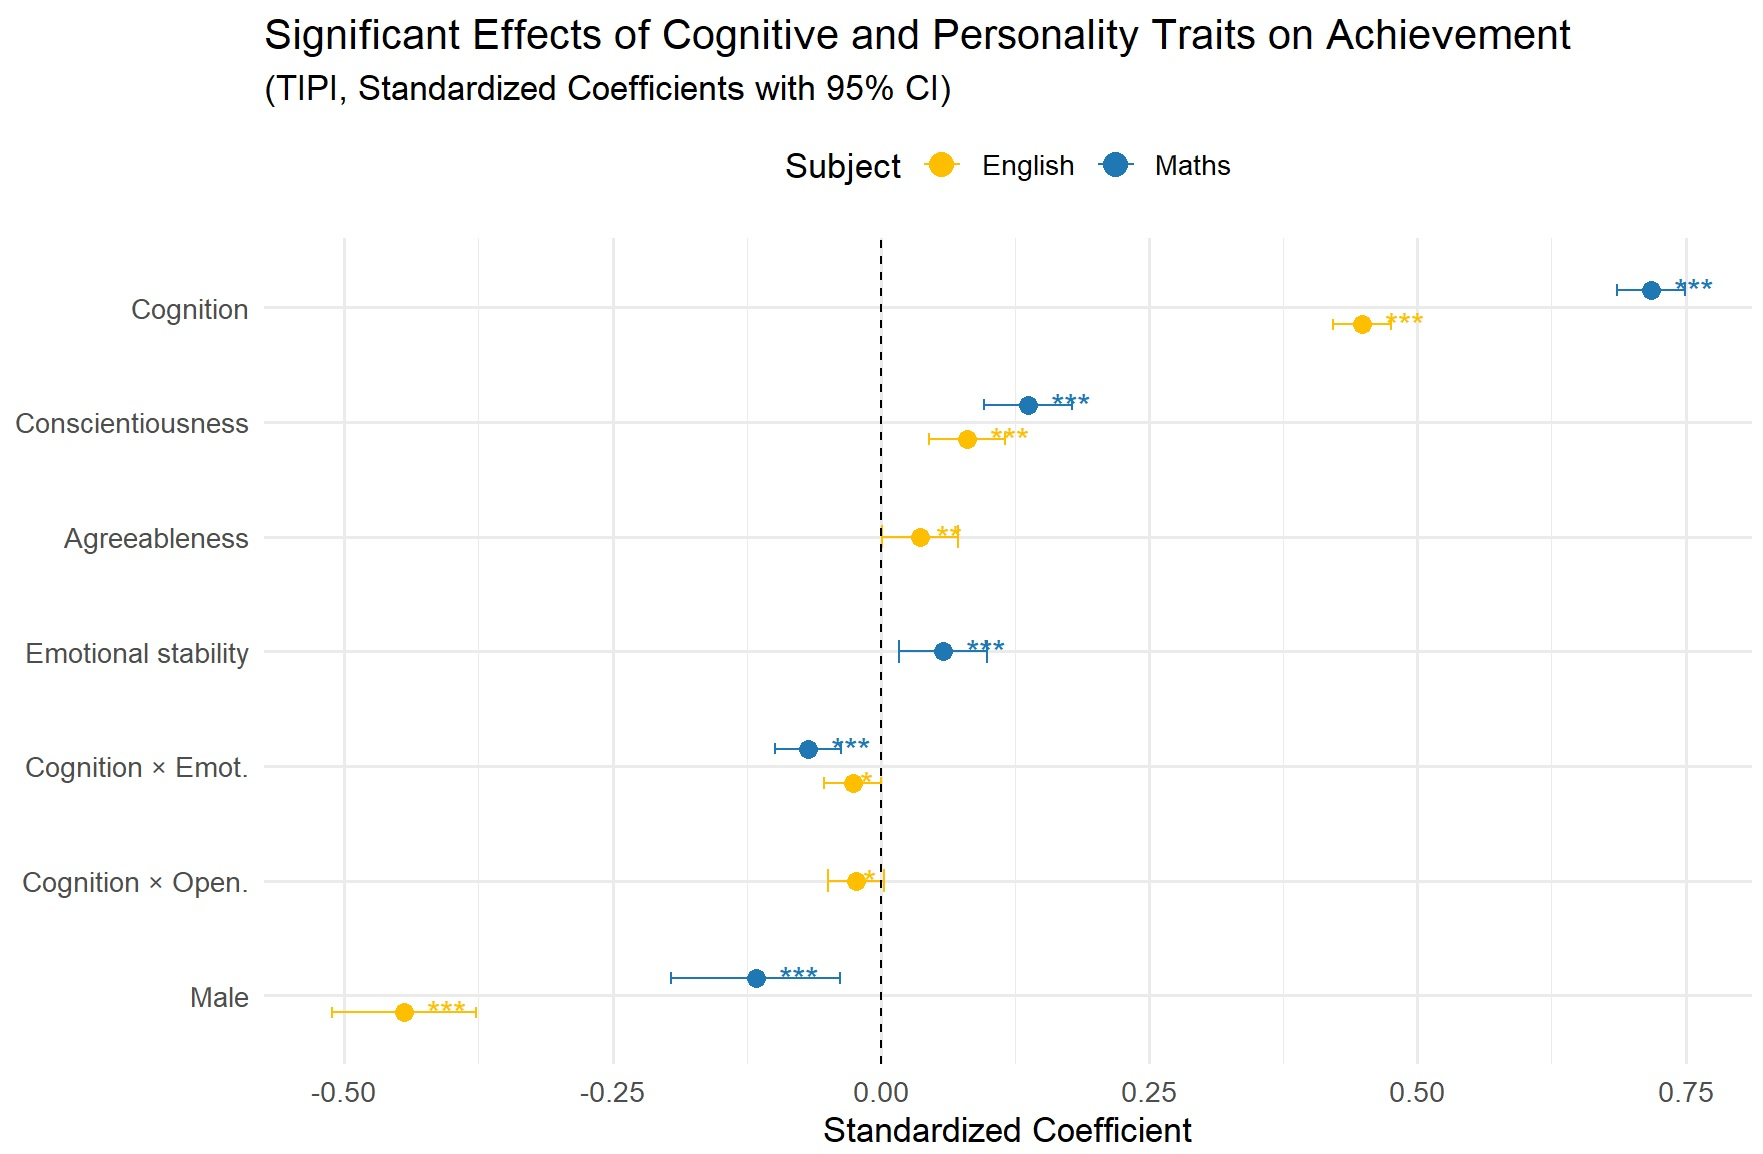
\includegraphics[width=0.9\linewidth]{TIPI_Linear_Estimates.JPG}
\end{figure}
\end{frame}

\begin{frame}{Results - Linear Estimation - SDQ}
\begin{figure}[h!]
    \centering
    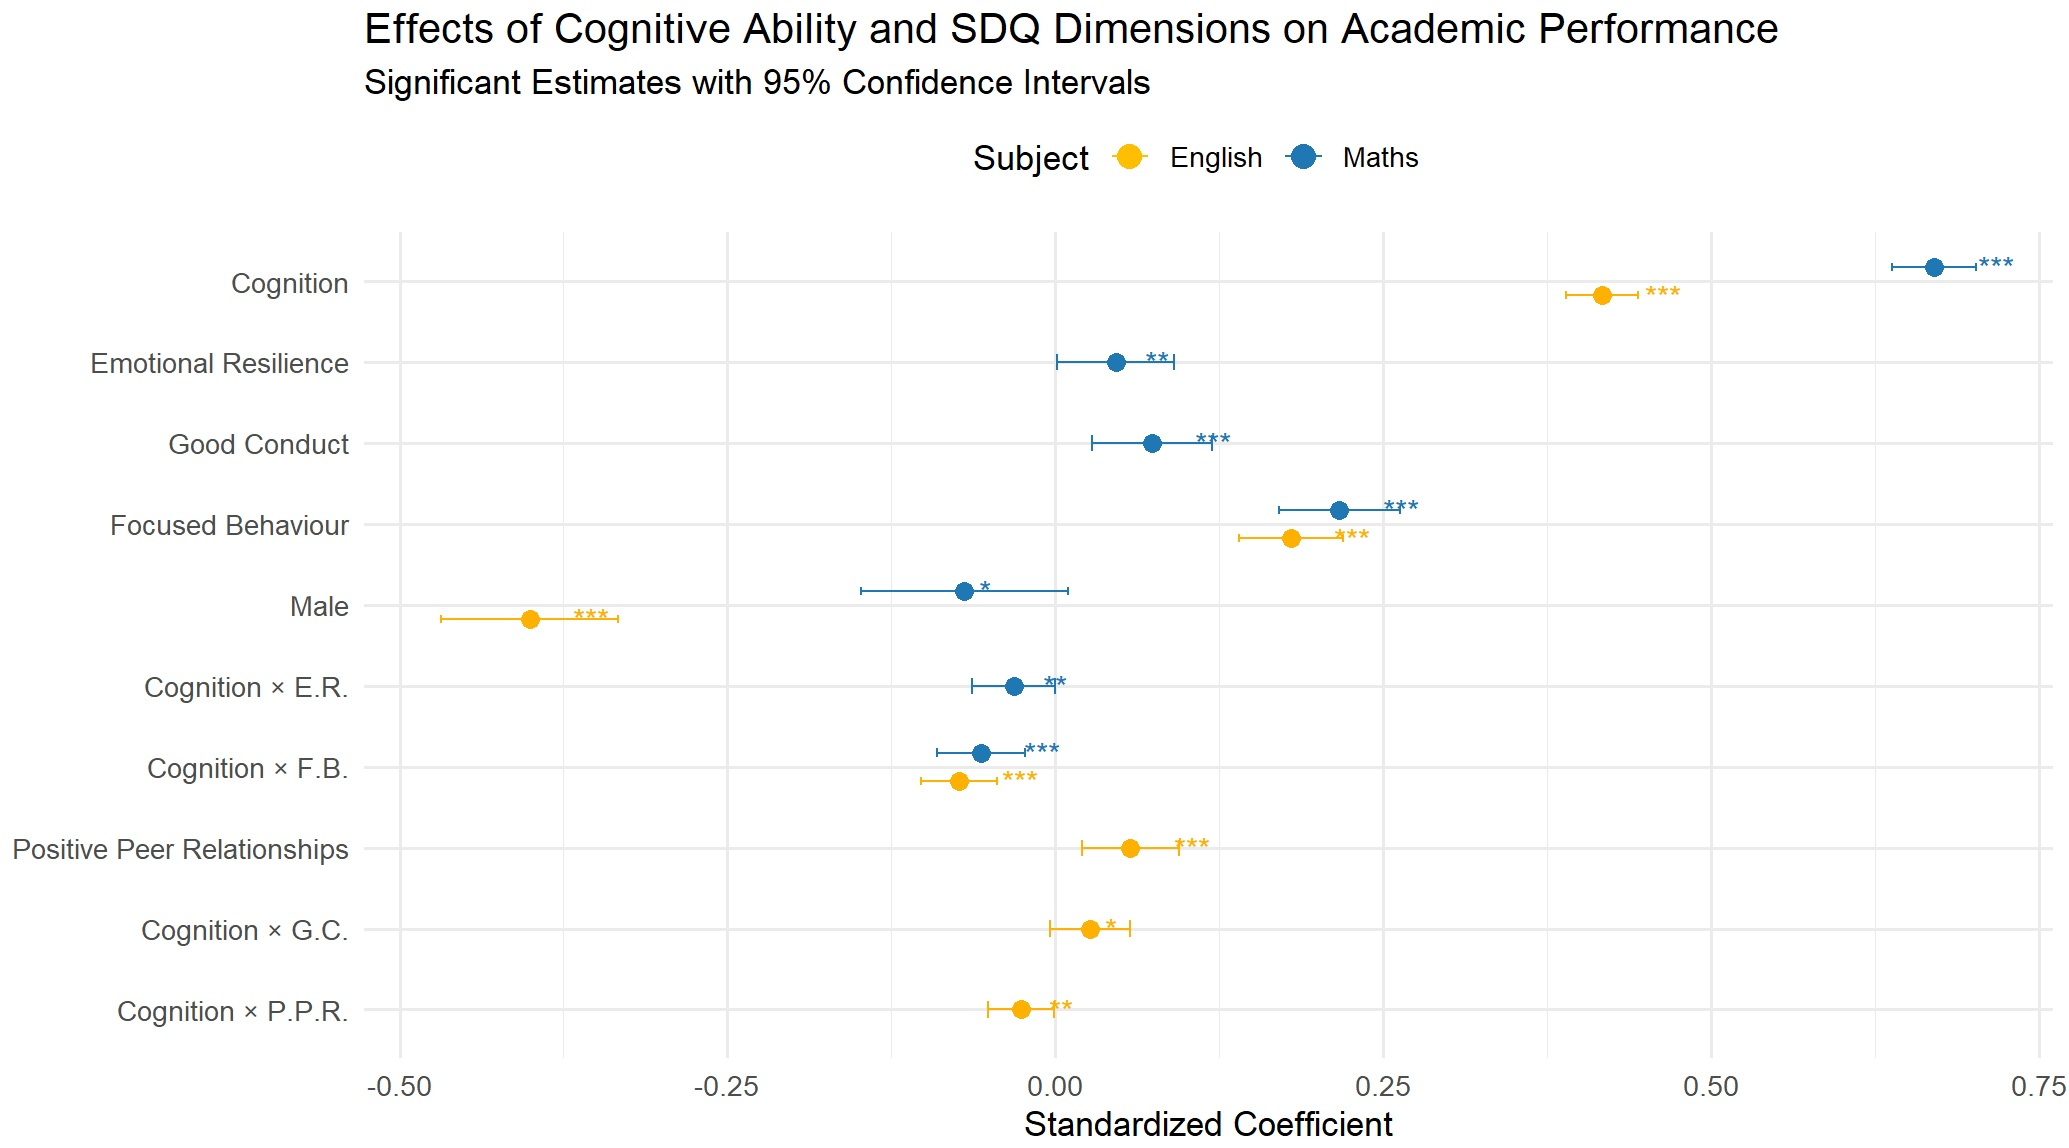
\includegraphics[width=1\linewidth]{SDQ_Linear_Estimates.JPG}
    \label{fig:your_label}
\end{figure}
\end{frame}

\begin{frame}{Discussion - Linear Estimation}

\begin{itemize}
\item \textbf{Cognitive Skills:} Strongest predictor of academic performance; one SD increase yields +0.67 (SDQ) to +0.72 (TIPI) points in Maths and +0.42 (SDQ) to +0.45 (TIPI) points in English.
    
    \item \textbf{Noncognitive Skills:} Focused Behaviour significantly boosts scores (+0.22 in Maths, +0.18 in English); Conscientiousness contributes modestly (+0.14 in Maths, +0.08 in English).

    \item \textbf{Interaction Effects:} Highly significant negative interactions between cognitive ability and noncognitive skill, which suggests importance for students with lower cognitive abilities.
    
    \item \textbf{Gender Differences:} Boys perform worse than girls, especially in English (-0.44 points); smaller gap in Maths (-0.12 points).

    \item \textbf{Subject Differences:} Cognitive skills have a stronger impact on Maths; noncognitive skills are more influential in English.
\end{itemize}
\end{frame}

    

\begin{frame}{Nonlinear Estimation: Translog P.F.}
\textbf{Equation:}
\begin{equation*}
Y = A C^{\alpha} N^{\beta} \exp\left\{ \frac{1}{2} \gamma_{1} \left[\ln(C)\right]^2 + \frac{1}{2} \gamma_{2} \left[\ln(N)\right]^2 + \gamma_{12} \ln(C) \ln(N) \right\}
\end{equation*}
\small
\textbf{Where:}
\begin{itemize}
    \item $Y$: Output (JC scores in Maths/English); $C$: Cognitive input (PC, $\mu$ = 100, $\sigma$ = 15); $N$: Noncognitive input (Focused Behaviour or Conscientiousness, original scales)
    \item $\alpha$, $\beta$: Output elasticities with respect to $C$ and $N$
    \item $\gamma_1$, $\gamma_2$, $\gamma_{12}$: Capture curvature and input interactions. A negative $\gamma_{12}$ implies diminishing marginal returns when both $C$ and $N$ are high.
\end{itemize}

The translog production function allows for variable elasticities of substitution and nonlinear input interactions. As a flexible second-order approximation, it extends beyond traditional models (e.g., Cobb-Douglas) and accommodates richer input-output relationships.
\end{frame}



\begin{frame}{Results - Nonlinear Estimation - Maths}

\begin{figure}[h!]
    \centering
    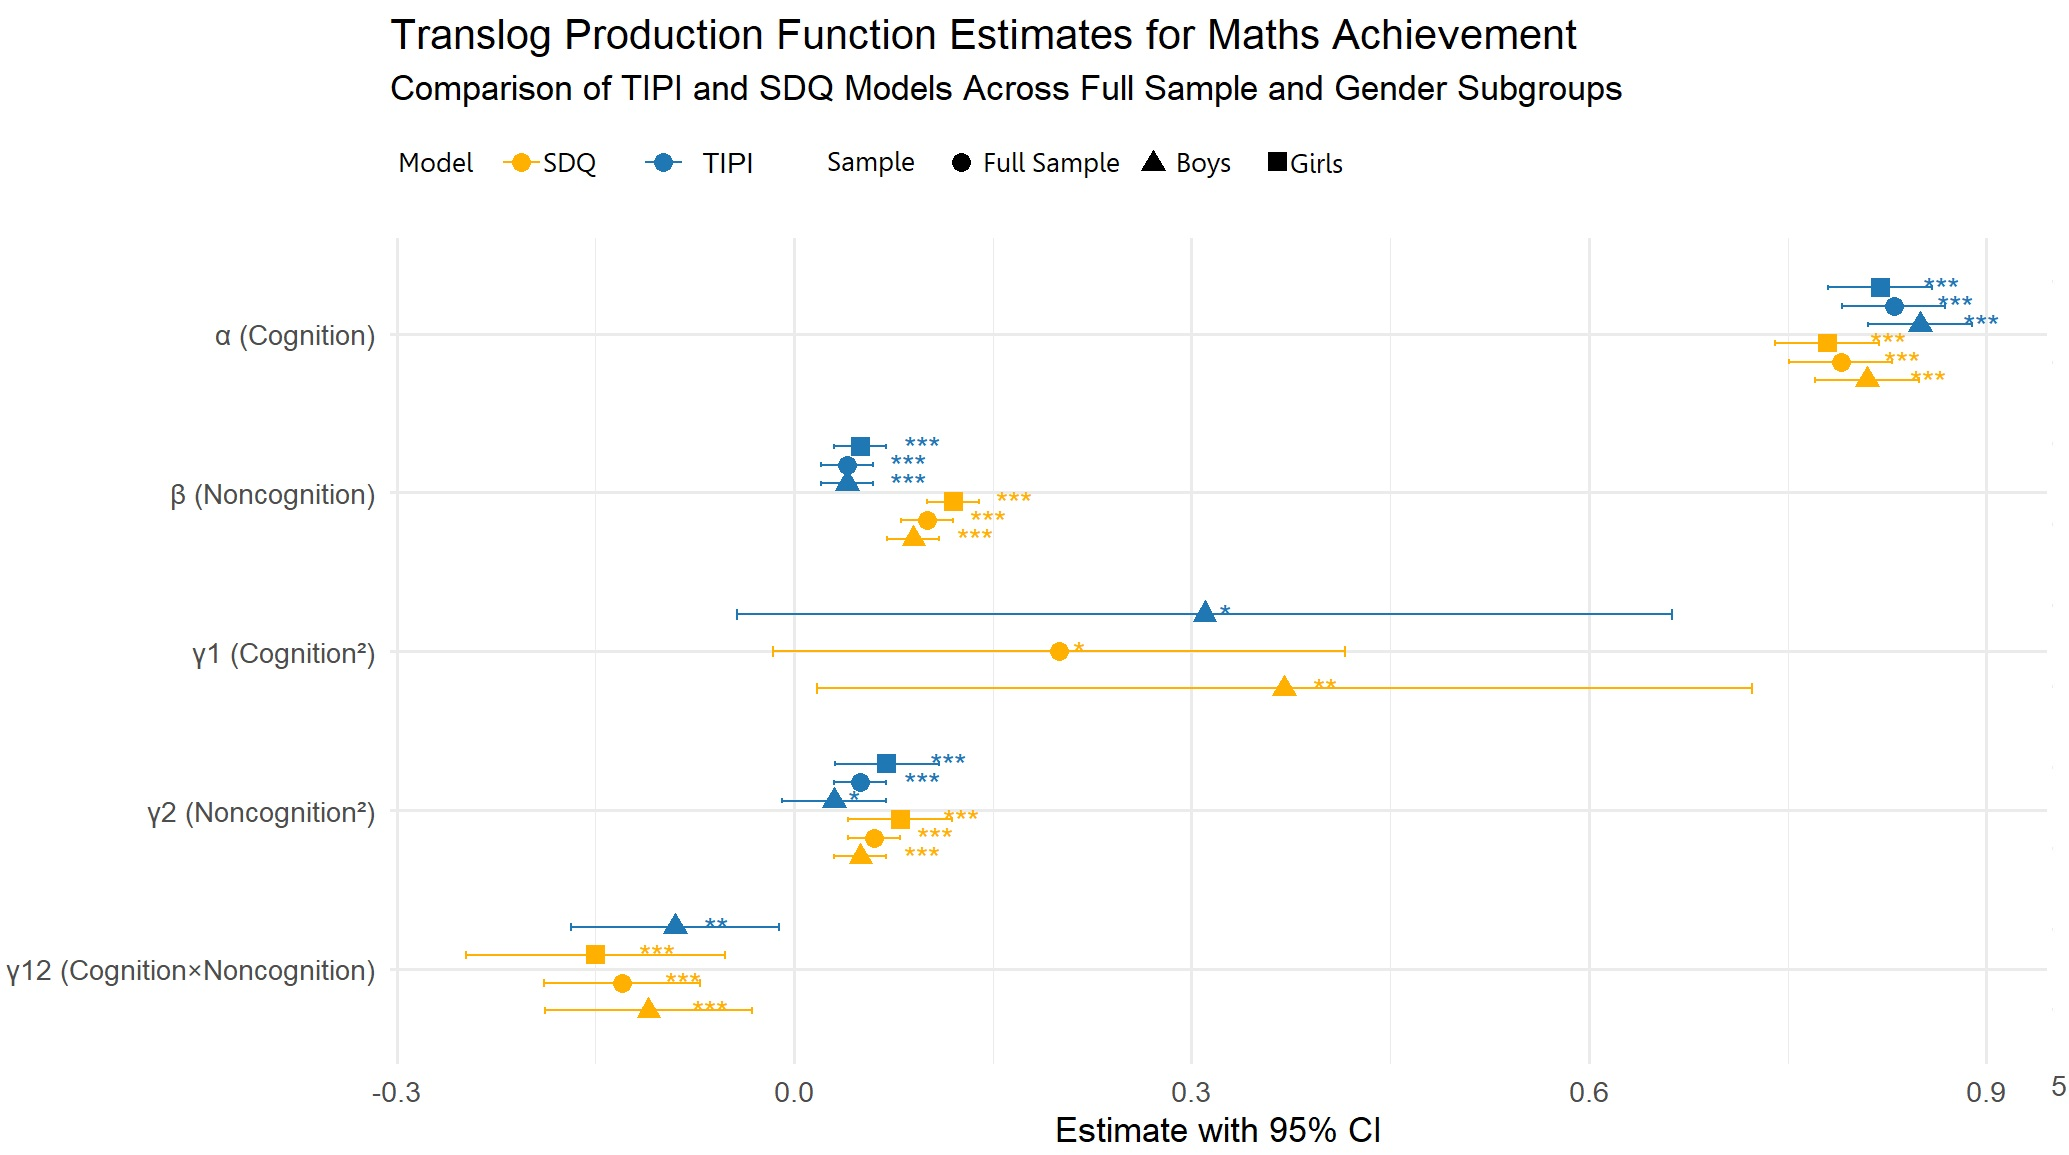
\includegraphics[width=1\linewidth]{Maths_Translog_Results.JPG}
    \label{fig:your_labelz}
\end{figure}
    \end{frame}

\begin{frame}{Results - Nonlinear Estimation - English}

\begin{figure}[h!]
    \centering
    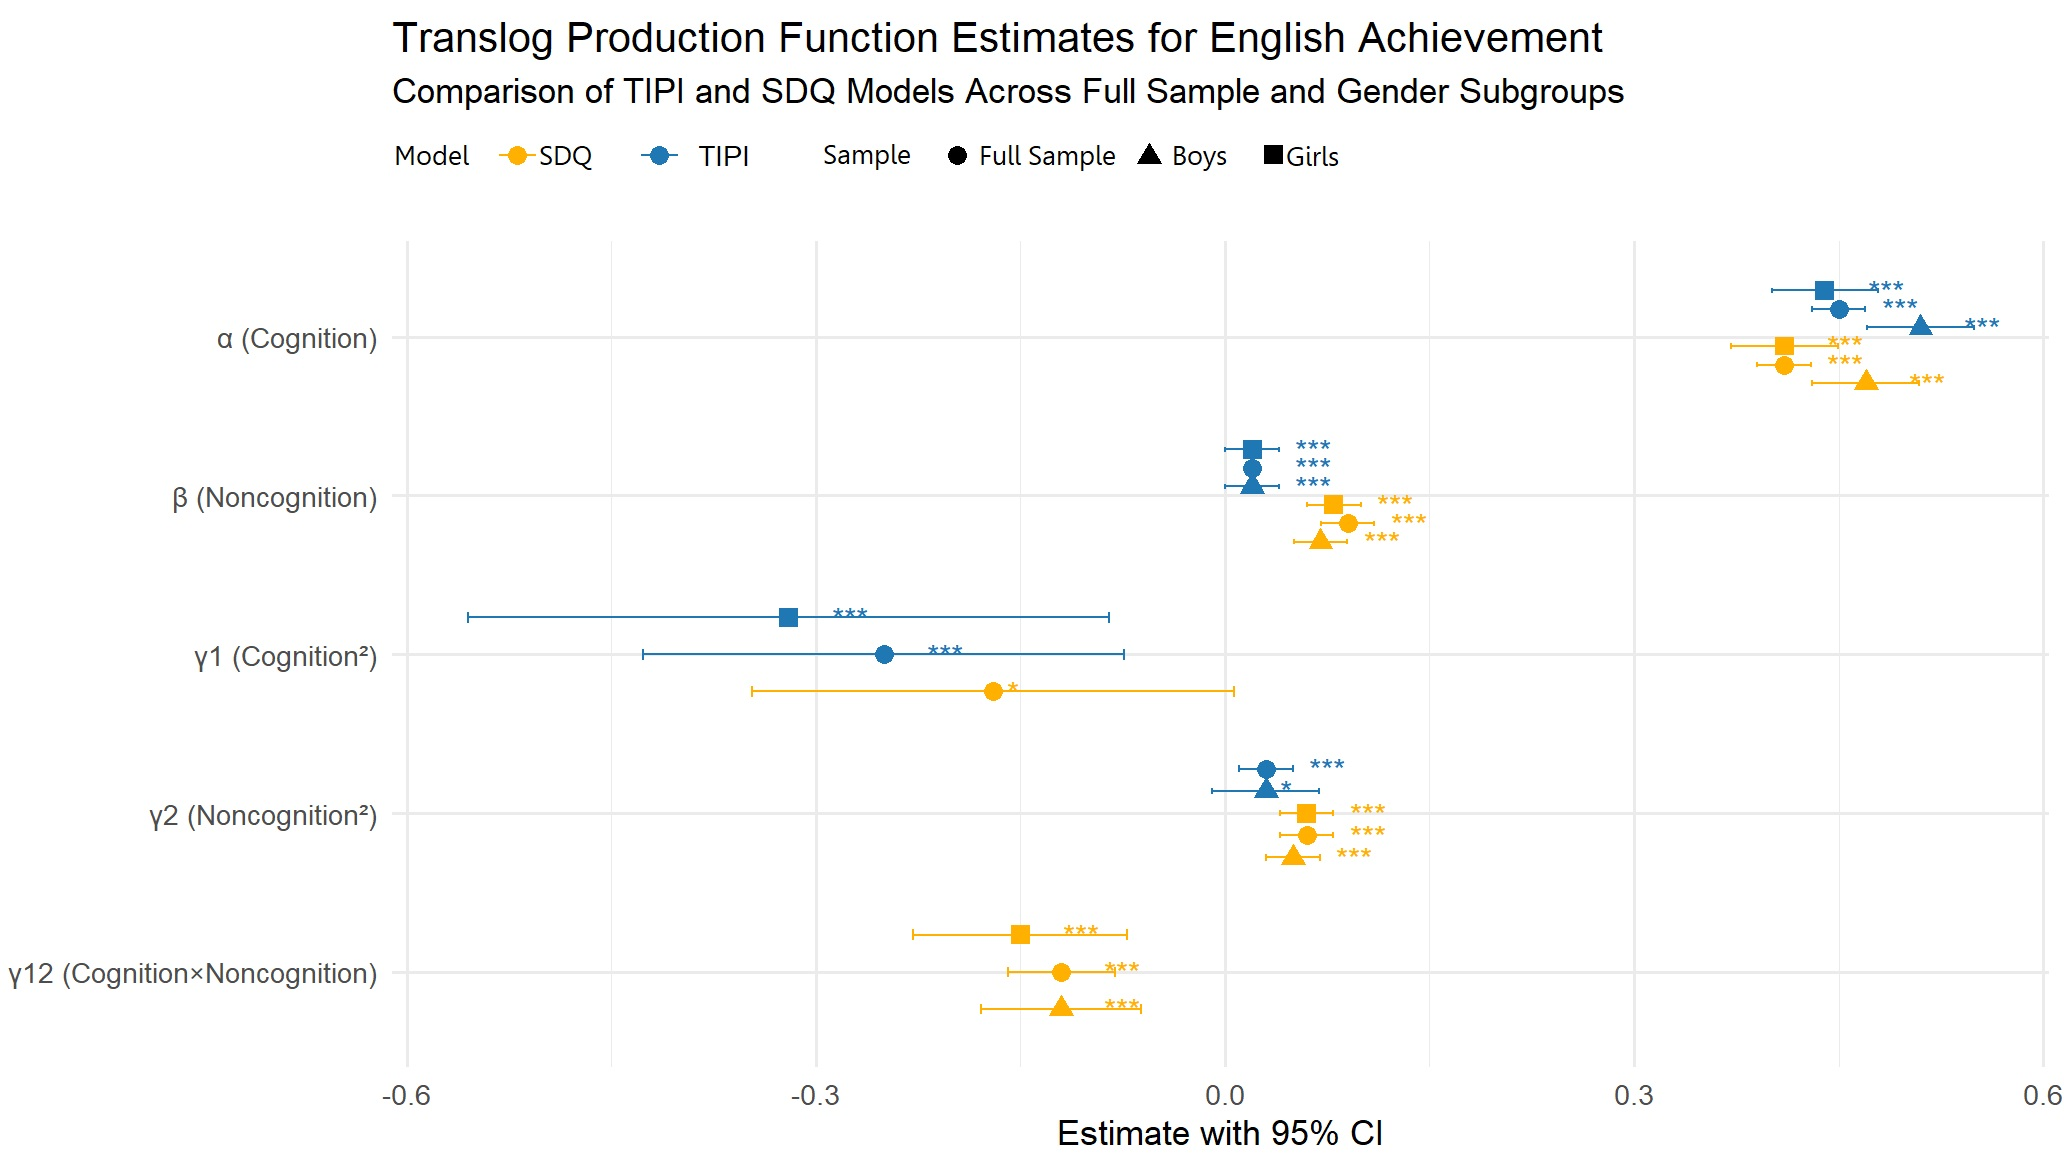
\includegraphics[width=1\linewidth]{English_Translog_Results.JPG}
    \label{fig:your_label}
\end{figure}
    \end{frame}


\begin{frame}{Discussion - Nonlinear Estimation}
\small
\begin{itemize}
    \item \textbf{Cognitive Skills ($\alpha$):} Strong influence on performance; $\alpha$ = 0.79 (SDQ, Maths) and 0.83 (TIPI, Maths) vs. $\alpha$ = 0.41 (SDQ, English) and 0.45 (TIPI, English). 
    \item \textbf{Noncognitive Skills ($\beta$):} Smaller but significant contributions; $\beta$ = 0.11 (Maths, SDQ) vs. $\beta$ = 0.09 (English, SDQ); TIPI values lower at 0.04 (Maths) and 0.02 (English).
    \item \textbf{Interaction Effects ($\gamma_{12}$):} Negative and significant for SDQ ($\gamma_{12} = -0.13$ for Maths, $-0.12$ for English), suggesting that the marginal effect of one input decreases as the level of the other increases — consistent with diminishing returns when both skills are high.
\end{itemize}
\end{frame}   

\begin{frame}{Discussion - Nonlinear Estimation}    
\begin{itemize}
    \item \textbf{Gender Differences:} Cognitive skills impact varies; girls: $\alpha = 0.778$ (Maths, SDQ), boys: $\alpha = 0.806$ (Maths, SDQ). Noncognitive skills are higher for girls in both subjects.
    \item \textbf{Measurement Tool Impact:} SDQ measures show stronger relationships with outcomes than TIPI, suggesting better relevance for academic performance.
\end{itemize}
\end{frame}


\begin{frame}{Results - Nonlinear Estimation}
\hypertarget{NonlinearEstimation}{}
\centering
\tiny
\renewcommand{\arraystretch}{1.2}
\setlength{\tabcolsep}{4pt}
\begin{tabular}{l|>{\columncolor{gray!20}}c>{\columncolor{gray!20}}c>{\columncolor{gray!20}}c|ccc}
\toprule
\rowcolor{gray!30}
& \multicolumn{3}{c|}{\textbf{Maths}} & \multicolumn{3}{c}{\textbf{English}} \\
\cmidrule{2-7}
\rowcolor{gray!30}
\textbf{Estimate} & \textbf{Full} & \textbf{Boys} & \textbf{Girls} & \textbf{Full} & \textbf{Boys} & \textbf{Girls} \\
\midrule
\multicolumn{7}{l}{\textbf{TIPI Model}} \\
\midrule
MP (Cognition) & 0.078 & 0.080 & 0.078 & 0.046 & 0.049 & 0.047 \\
MP (Conscientiousness) & 0.084 & 0.073 & 0.091 & 0.051 & 0.041 & 0.035 \\
OE ($\alpha$ Cognition) & 0.828 & 0.859 & 0.820 & 0.454 & 0.506 & 0.447 \\
OE ($\beta$ Conscientiousness) & 0.043 & 0.036 & 0.048 & 0.024 & 0.019 & 0.017 \\
EoS & 0.533 & 0.288 & 1.096 & 0.478 & 0.344 & 0.675 \\
MRTS & 0.927 & 1.102 & 0.858 & 0.894 & 1.217 & 1.342 \\
\midrule
\multicolumn{7}{l}{\textbf{SDQ Model}} \\
\midrule
MP (Cognition) & 0.074 & 0.076 & 0.074 & 0.042 & 0.045 & 0.043 \\
MP (Focused Behaviour) & 0.123 & 0.103 & 0.140 & 0.110 & 0.088 & 0.095 \\
OE ($\alpha$ Cognition) & 0.785 & 0.813 & 0.778 & 0.414 & 0.466 & 0.416 \\
OE ($\beta$ Focused Behaviour) & 0.105 & 0.084 & 0.125 & 0.088 & 0.069 & 0.078 \\
EoS & 0.471 & 0.451 & 0.488 & 0.452 & 0.396 & 0.370 \\
MRTS & 0.605 & 0.733 & 0.530 & 0.379 & 0.513 & 0.455 \\
\bottomrule
\end{tabular}

\vspace{0.3em}
\scriptsize
Note: MP = Marginal Product, OE = Output Elasticity, EoS = Elasticity of Substitution, \\
MRTS = Marginal Rate of Technical Substitution.
\vfill
\hfill
\hyperlink{Key Concepts}{\beamerbutton{Definitions}}

\end{frame}


\begin{frame}{Discussion - Nonlinear Estimation}
\small
\begin{itemize}
    \item \textbf{Higher Marginal Products (MPs):} Both cognitive and noncognitive skills yield greater returns in Maths than in English (particularly in the SDQ model)
    
    \item \textbf{Output Elasticities (OEs):} Cognitive skills remain the dominant drivers of achievement across subjects and genders, but noncognitive traits contribute meaningfully, particularly for girls in Maths.
    
    \item \textbf{Elasticity of Substitution (ES):} Estimates consistently below 1 indicate limited substitutability between skill types, except for girls in Maths (TIPI model: ES = 1.096), suggesting greater substitutability in this subgroup.
    
    \item \textbf{Marginal Rate of Technical Substitution (MRTS):} MRTS values below 1 in most models suggest that increasing noncognitive skills alone cannot fully offset deficits in cognitive skills.
    
    \item \textbf{Decreasing Returns to Scale:} The sum of $\alpha + \beta$ remains below 1 across all models, indicating diminishing returns to combined skill investments (a hallmark of constrained educational production).
\end{itemize}
\end{frame}



\begin{frame}{Conclusion}
\small
\begin{itemize}
    \item \textbf{Focus of Study:} Examined interactions of cognitive and noncognitive skills on academic achievement in Maths and English, highlighting gender differences.
    
    \item \textbf{Cognitive Skills:} Consistently the strongest predictor of performance, particularly influential in Maths across all models.
    
    \item \textbf{Noncognitive Skills:} Show meaningful but smaller effects; Focused Behaviour has a stronger impact in Maths, especially for girls (SDQ model).
    
    \item \textbf{Gender Differences:} Boys exhibit higher cognitive output elasticities; girls show greater substitutability between skills and stronger returns to noncognitive traits in some subjects.
    
    \item \textbf{Model Insights:} The translog specification reveals nonlinearities, interaction effects, and varying elasticity of substitution, offering richer insight than linear models.
    
    \item \textbf{Policy Implications:} Effective interventions should integrate both skill types and be tailored by subject and gender, given the observed differences in how students convert skills into achievement.
\end{itemize}
\end{frame}

\begin{frame}{Takeaways}

$\rightarrow$ Cognitive skills matter most for academic success—especially in Maths.

$\rightarrow$ But noncognitive traits, like focused behaviour, consistently boost outcomes, particularly for girls.

$\rightarrow$ Cognition and behaviour work best together: they are complements in most cases (ES $<$ 1), not substitutes $\rightarrow$ these skills do not easily replace each other. Students need support in both areas.

$\rightarrow$ To boost achievement, strategies should match students’ needs by subject, by skill, and by gender.
\end{frame}


\begin{frame}{Conclusion}
\begin{center}
Thank you so much.\\
Any questions or suggestions? \\
\textbf{b.gietner@gmail.com}

\begin{figure}[h!]
    \centering
    
\includegraphics[width=0.3\linewidth]{QR_Code.JPG}
    \label{fig:your_label}
\end{figure}



\end{center}
    
\end{frame}

\begin{frame}
\frametitle{Descriptive Statistics - Main Variables}
\hypertarget{MainVariables}{}
\tiny
\begin{table}
\centering
\caption{Descriptive Statistics - Main Variables}
\label{tab:main_desc_stats}
\begin{tabular}{lrrrrr}
\toprule
Variable & Mean & Std. Dev. & Min & Max & N \\
\midrule
\multicolumn{6}{l}{\textbf{Dependent variables}} \\
Maths points (Junior Cert) & 9.60 & 1.74 & 2.00 & 12.00 & 5631 \\
English points (Junior Cert) & 10.15 & 1.34 & 5.00 & 12.00 & 5631 \\
\midrule
\multicolumn{6}{l}{\textbf{Independent variables: Cognition}} \\
Drumcondra Verbal Reasoning (\% of correct answers) & 64.89 & 21.92 & 0.00 & 100.00 & 5631 \\
Drumcondra Numerical Ability (\% of correct answers) & 55.05 & 22.53 & 0.00 & 100.00 & 5631 \\
Matrices (BSA) & 116.68 & 18.03 & 10.00 & 161.00 & 5631 \\
Cognitive ability 1 & 0.14 & 1.33 & -4.25 & 3.32 & 5631 \\
Cognitive ability 2 & 100.00 & 15.00 & 36.25 & 136.40 & 5631 \\
\midrule
\multicolumn{6}{l}{\textbf{Independent variables: Noncognition (SDQ scale)}} \\
Emotional resilience & 8.29 & 1.87 & 0.00 & 10.00 & 5631 \\
Good conduct & 8.97 & 1.31 & 0.00 & 10.00 & 5631 \\
Focused behaviour & 7.56 & 2.26 & 0.00 & 10.00 & 5631 \\
Positive peer relationships & 8.96 & 1.41 & 0.00 & 10.00 & 5631 \\
\midrule
\multicolumn{6}{l}{\textbf{Independent variables: Noncognition (TIPI scale)}} \\
Agreeable & 5.01 & 1.95 & 0.50 & 7.00 & 5631 \\
Conscientious & 4.33 & 2.07 & 0.50 & 7.00 & 5631 \\
Emotional stability & 4.40 & 1.99 & 0.50 & 7.00 & 5631 \\
Extravert & 3.98 & 1.98 & 0.50 & 7.00 & 5629 \\
Openness & 4.73 & 1.83 & 0.50 & 7.00 & 5627 \\
\bottomrule
\end{tabular}
\end{table}
\vfill
\hfill
\hyperlink{Timeline}{\beamerbutton{Back}}
\end{frame}

% Control variables and notes slide
\begin{frame}
\frametitle{Descriptive Statistics - Control Variables}
\hypertarget{ControlVariables}{}
\tiny
\begin{table}
\centering
\caption{Descriptive Statistics - Control Variables}
\label{tab:control_desc_stats}
\begin{tabular}{lrrrrr}
\toprule
Variable & Mean & Std. Dev. & Min & Max & N \\
\midrule
\multicolumn{6}{l}{\textbf{Controls (SES characteristics)}} \\
Gender (Male = 1) & 0.49 & 0.50 & 0.00 & 1.00 & 5468 \\
Primary caregiver education level & 3.97 & 1.24 & 1.00 & 6.00 & 5631 \\
Secondary caregiver education level & 3.86 & 1.36 & 1.00 & 6.00 & 4440 \\
Income quintile (equivalized) & 3.33 & 1.39 & 1.00 & 5.00 & 5241 \\
\midrule
\multicolumn{6}{l}{\textbf{Controls (School characteristics, binary)}} \\
DEIS (Delivering Equality of Opportunity In Schools) & 0.12 & 0.33 & 0.00 & 1.00 & 5452 \\
Fee-paying & 0.10 & 0.30 & 0.00 & 1.00 & 5452 \\
Mixed-school & 0.54 & 0.50 & 0.00 & 1.00 & 5317 \\
\bottomrule
\end{tabular}
\end{table}
\vfill
\hfill
\hyperlink{Timeline}{\beamerbutton{Back}}
\end{frame}

\begin{frame}
\frametitle{Notes I}
\hypertarget{NotesI}{}
\tiny
\begin{itemize}
\item For the analysis, I used the Junior Certificate Overall Performance Scale (OPS), which converts letter grades from different exam levels to a standardized 12-point numerical scale. This scale has been validated in previous research by \href{https://www.jstor.org/stable/pdf/30077469.pdf}{Nick Sofroniou, Gerry Shiel and Judith Cosgrove (2000)}, and it provides a comprehensive measure that accounts for both grade and exam level.
\item TIPI scale scores on a 1-7 scale in intervals of 0.5, and the original SDQ scales, ranging from 0 to 10, have been inverted (higher scores typically indicate more problems on the original SDQ scale). 
\item "Cognitive ability 1" was used in the first part of the production function estimation and was standardized to have mean = 0 and standard deviation = 1. "Cognitive ability 2" is to be used in the second part of the analysis as a measure of cognition in non-linear production function estimation, with a mean of 100 and standard deviation = 15 as is standard in the literature. 
\item Education levels are coded from 1 (Primary or less) to 6 (Postgraduate/Higher degree) in the Growing Up in Ireland caregiver questionnaire. The mean values for both primary (3.97) and secondary (3.86) caregivers indicate an average education level between Leaving Certificate and Diploma/Certificate, suggesting a higher proportion of educated caregivers in the sample. 
\item Income is reported in quintiles, where 1 represents the lowest 20\% and 5 the highest 20\% of incomes. The mean of 3.33 suggests that the sample is slightly skewed towards higher income levels, with families on average being just above the median income quintile. \item The sample includes 12\% DEIS schools (schools in disadvantaged areas), 10\% fee-paying schools, and 54\% mixed-gender schools. This suggests a diverse range of school types, with a notably high proportion of fee-paying schools and a relatively low proportion of DEIS schools.
\end{itemize}
\vfill
\hfill
\hyperlink{Timeline}{\beamerbutton{Back}}
\end{frame}

\begin{frame}
\frametitle{Notes II}
\hypertarget{NotesII}{}

\begin{table}[htbp]
\tiny
\centering
\caption{Junior Certificate Overall Performance Scale (OPS)}
\label{tab:junior-cert-ops}
\begin{tabular}{|c|c|c|c|c}
\hline
Higher & Ordinary & Foundation & OPS \\
Level & Level & Level & Score \\
\hline
A & & & 12 \\
\hline
B & & & 11 \\
\hline
C & & & 10 \\
\hline
D & A & & 9 \\
\hline
E & B & & 8 \\
\hline
F & C & & 7 \\
\hline
& D & A & 6 \\
\hline
& E & B & 5 \\
\hline
& F & C & 4 \\
\hline
&   & D & 3 \\
\hline
&   & E & 2 \\
\hline
&   & F & 1 \\
\hline
\end{tabular}
\end{table}

\vfill
\hfill
\hyperlink{Timeline}{\beamerbutton{Back}}
\end{frame}

\begin{frame}{Key Concepts}
\hypertarget{Key Concepts}{}

\textbf{Marginal Products (MPs)} indicate how output changes with a small increase in one input, holding others constant. In the Translog model, these effects reflect not just the input level, but also how inputs interact.

\textbf{Output Elasticities (OEs)} capture the percentage change in output from a 1\% change in an input. Unlike linear models, Translog allows these elasticities to vary depending on input combinations.

\textbf{Marginal Rate of Technical Substitution (MRTS)} shows how much of one input is needed to offset a reduction in another. In Translog, this rate is flexible — adapting to student skill profiles.

\textbf{Elasticity of Substitution (ES)} measures how easily inputs can replace each other. Translog allows this substitutability to shift depending on the balance of skills.

\vfill
\hfill
\hyperlink{NonlinearEstimation}{\beamerbutton{Back}}
\end{frame}

\begin{frame}
\frametitle{Definitions}
\hypertarget{Definitions}{}
\tiny

\begin{equation}
MP_C = A \alpha C^{\alpha - 1} N_0^{\beta} \exp\left\{ \frac{1}{2} \gamma_{1} \left[\ln(C)\right]^2 + \frac{1}{2} \gamma_{2} \left[\ln(N_0)\right]^2 + \gamma_{12} \ln(C) \ln(N_0) \right\} \left[ \gamma_{1} \ln(C) \frac{1}{C} + \gamma_{12} \frac{\ln(N_0)}{C} \right]
\end{equation}

\begin{equation}
MP_N = A \beta C_0^{\alpha} N^{\beta - 1} \exp\left\{ \frac{1}{2} \gamma_{1} \left[\ln(C_0)\right]^2 + \frac{1}{2} \gamma_{2} \left[\ln(N)\right]^2 + \gamma_{12} \ln(C_0) \ln(N) \right\} \left[ \gamma_{2} \ln(N) \frac{1}{N} + \gamma_{12} \frac{\ln(C_0)}{N} \right]
\end{equation}

\begin{equation}
OE_C = \frac{\partial \ln(Y)}{\partial \ln(C)} \bigg|_{N=N_0} = \alpha + \gamma_{1} \ln(C) + \gamma_{12} \ln(N_0)
\end{equation}

\begin{equation}
OE_N = \frac{\partial \ln(Y)}{\partial \ln(N)} \bigg|_{C=C_0} = \beta + \gamma_{2} \ln(N) + \gamma_{12} \ln(C_0)
\end{equation}

\begin{equation}
MRTS_{CN} = \frac{\alpha + \gamma_{1} \ln(C) + \gamma_{12} \ln(N)}{\beta + \gamma_{2} \ln(N) + \gamma_{12} \ln(C)} \cdot \frac{N}{C}
\end{equation}

\begin{equation}
\sigma = \frac{OE_C + OE_N}{OE_C + OE_N - \gamma_{12}\left(\frac{OE_C}{OE_N} + \frac{OE_N}{OE_C}\right)}
\end{equation}
\vfill
\hfill
\hyperlink{NonlinearEstimation}{\beamerbutton{Back}}
\end{frame}



\begin{frame}{Theoretical Explanations for Negative Interaction}

    \begin{itemize}
        \item \textbf{Skill Complementarity with Diminishing Returns}: Skills enhance each other but with decreasing marginal effects at higher levels (Heckman, Stixrud, \& Urzua, 2006)
        \item \textbf{Self-Regulatory Resource Theory}: Brain has finite self-regulatory resources; allocation efficiency varies by skill profile (Blair \& Raver, 2015)
        \item \textbf{Developmental Compensation Hypothesis}: Students develop compensatory strategies that are especially valuable when one skill domain is weaker (Duckworth \& Seligman, 2005)
        \item \textbf{Specialized Skill Utilization}: Students with balanced high skills may not fully utilize both simultaneously in standard academic tasks (Almlund et al., 2011)
    \end{itemize}
\end{frame}

% Slide 2: Economic and Policy Implications
\begin{frame}{Economic and Policy Implications}
    \begin{itemize}
        \item \textbf{Human Capital Formation Models}: Negative interactions suggest optimal investment strategies should be personalized based on existing skill profiles (Heckman \& Kautz, 2012)
        \item \textbf{Critical Periods in Skill Development}: Different skill types may have distinct developmental windows, affecting their interaction efficiency (Moffitt et al., 2011)
        \item \textbf{Differential Returns by Context}: The substitutability between skill types varies by academic domain and demographic factors (Duckworth \& Gross, 2014)
        \item \textbf{Policy Implications}: Educational interventions should target specific skill deficits rather than applying uniform approaches; optimal strategy depends on both subject domain and student characteristics
    \end{itemize}
\end{frame}

\begin{frame}{Neurological Perspectives and Implications}
    \begin{itemize}
        \item \textbf{Neural Efficiency Hypothesis}: Different skill profiles show distinct patterns of brain activation; negative interaction reflects different neural strategies (Posner \& Rothbart, 2007)
        \item \textbf{Integration of Emotional and Cognitive Systems}: Neurobiological integration explains trade-offs between skill types (Immordino-Yang \& Damasio, 2007)
        \item \textbf{Executive Function as Mediator}: Executive functions mediate how cognitive abilities translate to performance (Zelazo, Blair, \& Willoughby, 2016)
    \end{itemize}
\end{frame}

% Reference slide (optional)
\begin{frame}[allowframebreaks]{References}
    \footnotesize
    \begin{thebibliography}{99}
        \bibitem{almlund} Almlund, M., Duckworth, A. L., Heckman, J. J., \& Kautz, T. (2011). Personality Psychology and Economics. \textit{In Handbook of the Economics of Education, Vol. 4}, 1--181.
        \bibitem{blair} Blair, C., \& Raver, C. C. (2015). School Readiness and Self-Regulation: A Developmental Psychobiological Approach. \textit{Annual Review of Psychology, 66}, 711--731.
        \bibitem{diamond} Diamond, A. (2013). Executive functions. \textit{Annual Review of Psychology, 64}, 135-168.
        \bibitem{duckworth2013} Duckworth, A. L., \& Carlson, S. M. (2013). Self-regulation and school success. \textit{Self-regulation and autonomy: Social and developmental dimensions of human conduct}, 208-230.
        \bibitem{duckworth2005} Duckworth, A. L., \& Seligman, M. E. P. (2005). Self-Discipline Outdoes IQ in Predicting Academic Performance of Adolescents. \textit{Psychological Science, 16}(12), 939--944.
        \bibitem{duckworth2014} Duckworth, A. L., \& Gross, J. J. (2014). Self-Control and Grit: Related but Separable Determinants of Success. \textit{Current Directions in Psychological Science, 23}(5), 319--325.
        \bibitem{heckman2006} Heckman, J. J., Stixrud, J., \& Urzua, S. (2006). The Effects of Cognitive and Noncognitive Abilities on Labor Market Outcomes and Social Behavior. \textit{Journal of Labor Economics, 24}(3), 411--482.
        \bibitem{heckman2012} Heckman, J. J., \& Kautz, T. (2012). Hard Evidence on Soft Skills. \textit{Labour Economics, 19}(4), 451--464.
        \bibitem{immordino} Immordino-Yang, M. H., \& Damasio, A. (2007). We feel, therefore we learn: The relevance of affective and social neuroscience to education. \textit{Mind, Brain, and Education, 1}(1), 3-10.
        \bibitem{moffitt} Moffitt, T. E. et al. (2011). A Gradient of Childhood Self-Control Predicts Health, Wealth, and Public Safety. \textit{Proceedings of the National Academy of Sciences, 108}(7), 2693--2698.
        \bibitem{posner} Posner, M. I., \& Rothbart, M. K. (2007). Research on attention networks as a model for the integration of psychological science. \textit{Annual Review of Psychology, 58}, 1-23.
        \bibitem{zelazo} Zelazo, P. D., Blair, C. B., \& Willoughby, M. T. (2016). Executive function: Implications for education. \textit{NCER 2017-2000}, National Center for Education Research.
    \end{thebibliography}
\end{frame}

\end{document}    
